\documentclass[9pt,journal]{IEEEtran}
\usepackage[utf8]{inputenc}
\usepackage{cite}
\usepackage[hidelinks]{hyperref}
\usepackage[shortlabels]{enumitem}

% Math
\usepackage{amsmath}
\DeclareMathOperator\erfc{erfc}
\usepackage{nicefrac}
% For tables
\usepackage[table]{xcolor}
\usepackage{tabularx, booktabs}
\usepackage{multirow}

% Units
\usepackage{siunitx}
\sisetup{
    exponent-product = \cdot,
    separate-uncertainty = true,
    per-mode = symbol,
    group-digits = false,
    detect-weight=true, 
    detect-family=true,
    detect-all
}
% Tikz
\usepackage[europeanresistors,americaninductors, americancurrents, american voltages, siunitx]{circuitikz}
\usepackage{tikz}
\usetikzlibrary{shapes,arrows, calc, automata, positioning, chains, decorations.markings, calc, patterns, angles, quotes}
\usepackage{pgfplots}

\usepackage{graphicx} % Figures/graphics
\usepackage{float} % Floats, H
% Subfigures:
\ifCLASSOPTIONcompsoc
    \usepackage[caption=false, font=normalsize, labelfont=sf, textfont=sf]{subfig}
\else
\usepackage[caption=false, font=footnotesize]{subfig}
\fi

% New commands
\newcommand{\ebnot}{$\nicefrac{E_b}{N_0}$}
\renewcommand{\Re}{\text{Re}}
\renewcommand{\Im}{\text{Im}}

% TODOs
\newcommand\todo[1]{\textcolor{red}{#1}}


% -------------------------------- System variables ----------------------------- %
% Specs

\newcommand{\MainCarrierFreq}{2415} %MHz
\newcommand{\paPower}{-10} % dBm
\newcommand{\BERThreshold}{$1\cdot10^{-2}$} % For changing quality
\newcommand{\BERPowerLimit}{-17} % dBm

\newcommand{\bitPerSymbQPSK}{2}
\newcommand{\bitPerSymbQAM}{4}
\newcommand{\soundSampleRateQPSK}{11025}
\newcommand{\soundSampleRateQAM}{22050}
\newcommand{\bitPerSoundSample}{12}


\newcommand{\headerBits}{8}
\newcommand{\packetDataSymbolsQPSK}{456}
\newcommand{\packetDataSymbolsQAM}{228}
\newcommand{\packetDataBitsQPSK}{512}
\newcommand{\packetDataBitsQAM}{512}

\newcommand{\barkerSymbols}{26}
\newcommand{\barkerBitsQPSK}{\the\numexpr2*\barkerSymbols\relax}
\newcommand{\barkerBitsQAM}{\the\numexpr4*\barkerSymbols\relax}

\newcommand{\guardSymbols}{2}
\newcommand{\guardBitsQPSK}{\the\numexpr\bitPerSymbQPSK*\guardSymbols\relax}
\newcommand{\guardBitsQAM}{\the\numexpr\bitPerSymbQAM*\guardSymbols\relax}
\newcommand{\burstLengthSymbolsQPSK}{484}
\newcommand{\burstLengthSymbolsQAM}{256}
\newcommand{\burstSizeBitsQPSK}{331}
\newcommand{\burstSizeBitsQAM}{935}

\newcommand{\systemBitRateQPSK}{187.39} % kbits/s
\newcommand{\systemBitRateQAM}{572.67} % kbits/s
\newcommand{\symbolRateQPSK}{150 } % ksymb/s
\newcommand{\symbolRateQAM}{\symbolRateQPSK} % ksymb/s
\newcommand{\filterRollOff}{0.5}
\newcommand{\sps}{8}


\newcommand{\minBWQPSK}{112,5}% kHz
\newcommand{\minBWQAM}{\minBWQPSK}% kHz
\newcommand{\maxSystemBW}{100} % kHz

% Data rates
\newcommand{\rawDataRate}{1.4} %Mb/s
\newcommand{\sourceDataRateQPSK}{\the\numexpr\bitPerSoundSample*\soundSampleRateQPSK/1000\relax} % kb/s
\newcommand{\sourceDataRateQAM}{\the\numexpr\bitPerSoundSample*\soundSampleRateQAM/1000\relax} % kb/s
\newcommand{\packetDataRateQPSK}{134.4} % kb/s
\newcommand{\packetDataRateQAM}{268.7} % kb/s
\newcommand{\fecDataRateQPSK}{235.1} % kb/s
\newcommand{\fecDataRateQAM}{470.3} % kb/s
\newcommand{\symbolMapRateQPSK}{117.6} % ksymb/s
\newcommand{\symbolMapRateQAM}{117.6} % ksymb/s
\newcommand{\barkerRateQPSK}{124.5} % ksymb/s
\newcommand{\barkerRateQAM}{130.2} % ksymb/s
\newcommand{\sampleRateQPSK}{1.00} % M sample/s
\newcommand{\sampleRateQAM}{1.06} % M sample/s

\newcommand{\USRPSampleRate}{1.2} %Msamp/s


% BER Feedback path
\newcommand{\BERDataBits}{26}
\newcommand{\BERBurstSize}{43} % Symbols

\newcommand{\BERCarrierFreq}{2455} %MHz
\newcommand{\BERSymbolRate}{\symbolRateQPSK} %ksymb/s
\newcommand{\BERminBW}{\minBWQPSK}


% ------------------------ MEASUREMENTS -----------------------------%
\newcommand{\measBW}{220.6} %kHz, -40dBc
\newcommand{\measPWR}{-10} %dBm
\newcommand{\measPWRbad}{-25} %dBm
\newcommand{\measDelay}{262} %ms
\newcommand{\measDelayStd}{63} %ms
\newcommand{\measDelaySwitch}{40} %ms

\newcommand{\measSNRQPSKGood}{18.1} %dB
\newcommand{\measSNRQAMGood}{12.8} %dB
\newcommand{\measSNRQPSKBad}{15.9} %dB
\newcommand{\measSNRQAMBad}{10.16} %dB
\newcommand{\measEVMGood}{-9} %dB
\newcommand{\measEVMBad}{-4} %dB
\newcommand{\measBERQPSKGood}{\SI{1.35e-6}{\;}} 
\newcommand{\measBERQAMGood}{\SI{6.0e-2}{\;}} 
\newcommand{\measBERQPSKBad}{\SI{1.4e-5}{\;}} 
\newcommand{\measBERQAMBad}{\SI{1.32e-1}{\;}} 


% ------------------------ Document Variables ---------------------------- % 
\newcommand{\figW}{0.7}



% ---------------------------------- DOCUMENT ------------------------------------------------- %

\title{Demonstration of Adaptable Quality Radio System for Broadcasting of Speech}
\author{Martin Lima and Fredrik Esp Feyling }
\date{April 2020}

\begin{document}

\maketitle
\begin{abstract} 
This paper is presenting the design and implementation of a radio communication system for broadcasting of speech with adaptable data rate. This system is to be seen as a "proof of concept", where the main goal is to demonstrate a radio system with feedback from receiver (RX) to transmitter (TX) such that the transmitted data rate adapts to the state of the radio channel. The data rate is varied by a factor 2 by switching between QPSK and QAM-16 modulation while bandwidth and transmit power are fixed. The proposed system is implemented with a \SI{-55}{dBc} bandwidth of \SI{\measBW}{\kilo\hertz} and a transmit power of \SI{\measPWR}{dBm}.

The adaptive quality feature is verified and the system changes quality immediately when the detected error rate drops below a predefined threshold. The measured bit error rates are \measBERQAMGood  and \measBERQPSKBad for high and low data rates respectively. The total delay from transmitter to receiver is measured to \SI{\measDelay}{\milli\second}, making the system well suited the for two-way communication as well as broadcasting. 
\end{abstract}

% INTRODUCTION
% !TEX root = main.tex
\section{Introduction}
\label{sec:Introduction}
When designing any radio communication system, trade-offs has to be made between bandwidth, power, system complexity and bit rate. For a given bandwidth and transmit power, the bit rate could be varied by using different modulation schemes. As higher order modulation schemes require higher $\frac{E_b}{N_0}$, choosing optimum modulation scheme would require knowledge about the radio channel in order to maintain low enough BER at the receiver. This knowledge may be obtained by adding complexity in form of a feedback channel from receiver to transmitter. By performing some kind of error detection, the receiver may send information about detected error rates back to the transmitter. This enables the system to adapt the data rate to the state of the radio channel, and thus provide better QoS for given power and bandwidth. 

In this paper, we present a radio communication system with this kind of feedback structure. The system is to be seen as a "proof of concept" and the goal is not to propose a complete radio system for commercial use. The adaptable quality is obtained by implementing a feedback path from the receiver to the transmitter, using frequency-division duplexing (FDD). Figure \ref{fig:block_toplevel} shows a top level block diagram of the proposed system. The figure shows that speech data is sent in the forward path from transmitter to receiver, and the number of detected errors is sent in the feedback path from receiver to transmitter. The forward and feedback paths will be referred to as the \textit{data path} and the \textit{BER path} respectively. 
% !TEX root = main.tex
\begin{figure}[htbp]
\centering
\begin{tikzpicture}[                
                    box/.style={
            		draw,
			thick,
            		text centered,
            		minimum width=1.5cm,
            		minimum height=1cm,
			font=\footnotesize,
			align=center,
			anchor=center,
            	} ]
	

\draw 
(0,0) node[box] (trans) {Transmitter}
(3,0) node[box] (rec) {Receiver}
(rec.west) ++(0,0.3) coordinate[](data_in) {}
(trans.east) ++(0,0.3) coordinate[](data_out) {}
(rec.west) ++(0,-0.3) coordinate[](ber_in) {}
(trans.east) ++(0,-0.3) coordinate[](ber_out) {}
;
\draw[thick, ->] (data_out) -- ++(0.8, -0.1) -- ++(-0.2, 0.2) node[above, align=center, font=\scriptsize, anchor=south, xshift=0.1cm]{Speech data} -- (data_in);
\draw[thick, <-] (ber_out) -- ++(0.8, -0.1) -- ++(-0.2, 0.2) node[below, align=center, font=\scriptsize, anchor=north, yshift=-0.1cm, xshift=0.1cm]{Detected \\ errors} -- (ber_in);

	
\end{tikzpicture}
\caption{Top level block diagram of proposed system. Speech data is sent in the forward path from transmitter to receiver and the number of detected errors is sent back from receiver to transmitter.}
\label{fig:block_toplevel}
\end{figure}. 

The proposed system is designed to switch between two different data rates, using two different modulation formats. Figure \ref{fig:concept} shows a qualitative illustration of the adaptive quality concept. The proposed system may be further improved by adding more levels, yielding even better utilization of available resources.

% !TEX root = main.tex
\begin{figure}[htbp]
\centering
\begin{tikzpicture}
% Coordinate system
\coordinate (origo) at (0,0);

\draw[->, thick] (-0.3, 0) -- (5, 0) node[below, font=\scriptsize]{SNR};
\draw[->, thick] (0, -0.3) -- (0, 3) node[left, align=center, font=\scriptsize]{bits/\\symbol};

\foreach \x in {1, 2, 3, 4, 5}
   \draw (1pt, 0.5*\x cm) -- (-1pt, 0.5*\x cm) node[anchor=east] {$\x$};
   
% \draw (2.5, 1pt) -- (2.5, -1pt) node[anchor=north] {$\left[\frac{E_b}{N_0}\right]$};

%Lines
\draw[] (0.6, 1) -- node[above, font=\scriptsize, xshift=-0.5cm]{QPSK} (2.5,1) -- (2.5, 2) -- node[above, font=\scriptsize]{QAM-16} (5, 2) node[below, xshift=0.2cm, align=center, font=\scriptsize](c2){Proposed \\ system}; 
\draw[dashed, blue] (0.6, 1) -- (1.7, 1) -- (1.7, 1.5) -- (3.2, 1.5) -- (3.2, 2) -- (4.5, 2) -- (4.5, 2.5) -- (5, 2.5) node[above, xshift=0.2cm, align=center, font=\scriptsize](c2){Future \\ improvement}; 

\draw plot [domain=0.1:5,samples=100] (\x,{log2(1 + 2.5*\x)});
\draw (2, 2.5) node[above, font=\scriptsize, rotate=33]{Shannon Limit};


\end{tikzpicture}
\caption{Qualitative illustration of the adaptive quality concept}
\label{fig:concept}
\end{figure}

Throughout this paper, we will use the word \textit{transmitter} when referring to the radio module that is transmitting the speech data and \textit{receiver} when referring to the module that is receiving it. This is not to be confused with the terms TX and RX, which we use when referring to the transmit and receive port on each radio module. 

The system is implemented using the software defined radio USRP-2901\cite{USRP2901} from National Instruments, which contains all necessary RF hardware. All the software parts of the system is implementing in C++ and is executed on a standard personal computer. Pre-written C-libraries are used for the parts of the system concerning interface to the USRP, the computer sound card etc. These parts will not be explained in detail, but references to the libraries will be given. For the remaining parts of the system, we focus on explaining the implementation on a behavioural level and detailed descriptions of C code implementations is avoided. 

In section \ref{sec:specifications} we present the system specifications and the link budget is presented in section \ref{sec:link_budget} together with associated measurements. A detailed description of the proposed system is given in section \ref{sec:design_description} and the motivation behind some crucial design decisions is presented in section \ref{sec:design_motivation}. Performed measurements is presented in section \ref{sec:verification} before a final conclusion is given in section \ref{sec:conclusion}.

% SPECIFICATIONS
% !TEX root = main.tex
\section{System Specifications}
\label{sec:specifications}
The proposed radio communication system switches between QPSK and QAM-16 modulation, at a fixed transmit power and bandwidth, in order to obtain adaptable sound quality.  The system use the 2.4GHz ISM band with a carrier frequency of 2.415GHz and 2.455GHz for the data path and BER path respectively. The system is designed for a transmission distance of 2 meter in an indoor environment.

Some key system specifications are listed in table \ref{tab:specs_data} and \ref{tab:specs_ber}. Table \ref{tab:specs_data} shows the parameters for the data path and the values are listed for low / high data rate transmission. Table \ref{tab:specs_ber} shows parameters for the simpler BER path. 
% !TEX root = main.tex
% Table generated by Excel2LaTeX from sheet 'specs'
\begin{table*}[htbp]
  \centering
  \caption{System specifications}
    \begin{tabular}{lcccrr}
    \rowcolor[rgb]{ 0,  0,  0} \multicolumn{1}{c}{\textcolor[rgb]{ 1,  1,  1}{\textbf{System Variables}}} & \textcolor[rgb]{ 1,  1,  1}{\textbf{Variable}} & \textcolor[rgb]{ 1,  1,  1}{\textbf{Units}} & \textcolor[rgb]{ 1,  1,  1}{\textbf{Equation}} & \multicolumn{2}{c}{\textcolor[rgb]{ 1,  1,  1}{\textbf{Value}}} \\
    \rowcolor[rgb]{ 0,  0,  0} \textcolor[rgb]{ 1,  1,  1}{} & \textcolor[rgb]{ 1,  1,  1}{} & \textcolor[rgb]{ 1,  1,  1}{} & \textcolor[rgb]{ 1,  1,  1}{} & \multicolumn{1}{c}{\textcolor[rgb]{ 1,  1,  1}{\textbf{Low Data Rate}}} & \multicolumn{1}{c}{\textcolor[rgb]{ 1,  1,  1}{\textbf{High Data Rate}}} \\
    Frequency & $f_0$ & MHz   &       & 2415  & 2415 \\
    Modulation &       &       &       & \multicolumn{1}{l}{QPSK} & \multicolumn{1}{l}{QAM64} \\
    Bit per symbol  & m     &       &       & 2     & 6 \\
    Sound sampling rate & $f_s$ & Hz    &       & 11025 & 22050 \\
    Bits per sound sample & $b_s$ & bits  &       & 8     & 12 \\
    Sound datarate & $R_{ss}$ & kbits/s & $f_s \cdot b_s$ & 88,2  & 264,6 \\
    Channel coding &       &       &       & \multicolumn{1}{l}{Hamming (4,7)} & \multicolumn{1}{l}{Hamming (4,7)} \\
    Channel coded data rate &       & bits  & $R_ss \cdot 7/4$ & 154,35 & 463,05 \\
    \rowcolor[rgb]{ 0,  0,  0} \textcolor[rgb]{ 1,  1,  1}{\textbf{Packet Parameters}} & \textcolor[rgb]{ 1,  1,  1}{} & \textcolor[rgb]{ 1,  1,  1}{} & \textcolor[rgb]{ 1,  1,  1}{} & \multicolumn{2}{c}{\textcolor[rgb]{ 1,  1,  1}{}} \\
    Packet header size  &       & bits  &       & \headerBits    & \headerBits \\
    Packet data length &       & symbols &       & \packetSataSymbols   & \packetSataSymbols \\
    Packet size &       & bits  &       & \packetDataBitsQPSK   & \packetDataBitsQPSK \\
    \rowcolor[rgb]{ 0,  0,  0} \textcolor[rgb]{ 1,  1,  1}{\textbf{Frame Parameters}} & \textcolor[rgb]{ 1,  1,  1}{} & \textcolor[rgb]{ 1,  1,  1}{} & \textcolor[rgb]{ 1,  1,  1}{} & \multicolumn{2}{c}{\textcolor[rgb]{ 1,  1,  1}{}} \\
    Training sequence type &       &       &       & \multicolumn{1}{l}{Barker} & \multicolumn{1}{l}{Barker} \\
    Training sequence length &       & symbols &       & \barkerSymbols    & \barkerSymbols \\
    Training sequence size bits &       & bits  &       & \frameSizeBitsQPSK    & \frameSizeBitsQAM \\
    Frame size &       & bits  &       & 319   & 935 \\
    \rowcolor[rgb]{ 0,  0,  0} \textcolor[rgb]{ 1,  1,  1}{\textbf{Burst Parameters}} & \textcolor[rgb]{ 1,  1,  1}{} & \textcolor[rgb]{ 1,  1,  1}{} & \textcolor[rgb]{ 1,  1,  1}{} & \multicolumn{2}{c}{\textcolor[rgb]{ 1,  1,  1}{}} \\
    Guard period &       & symbols &       & \guardSymbols     & \guardSymbols \\
    Burst size &       & bits  &       & \burstSizeBitsQPSK   & \burstSizeBitsQAM \\
    \rowcolor[rgb]{ 0,  0,  0} \textcolor[rgb]{ 1,  1,  1}{\textbf{Transmission Characteristics}} & \textcolor[rgb]{ 1,  1,  1}{} & \textcolor[rgb]{ 1,  1,  1}{} & \textcolor[rgb]{ 1,  1,  1}{} & \textcolor[rgb]{ 1,  1,  1}{} & \textcolor[rgb]{ 1,  1,  1}{} \\
    System bit rate & $R_b$ & kbits/s &       & \systemBitRateQPSK & \systemBitRateQAM \\
    Symbol rate & $R_s$ & ksymbols/s &       & \symbolRateQPSK & \symbolRateQAM \\
          &       &       &       &       &  \\
    Pulse shaping filter &       &       &       & \multicolumn{1}{l}{root raised cosine} & \multicolumn{1}{l}{root raised cosine} \\
    Pulse shaping filter parameter & $\alpha$ &       &       & 0,3   & 0,3 \\
    \textbf{Minimum signal bandwidth} & $\Delta f$ & kHz   &       & \textbf{\minBWQPSK} & \textbf{\minBWQAM} \\
    \end{tabular}%
  \label{tab:addlabel}%
\end{table*}%


The burst format for the transmitted data is shown in figure \ref{fig:burst_format}. The bursts are different when using QPSK and QAM-16 modulation, because the same number of training symbols maps to a different number of bits. The data packages (a and b) is transmitted continuously with the indicated guard period. The BER packages is very small compared to the data packages, and is only transmitted ones per received data package. Thus no guard period is specified for these packages. 
% !TEX root = main.tex
\begin{figure} 
    \centering
  \subfloat[QPSK data packet\label{1a}]{%
\begin{tikzpicture}[                
                    slot/.style={
            		text centered,
			font=\scriptsize,
			align=center,
			anchor=center,
			minimum height=0.7cm
            	}]
\draw[thick] (0,0) rectangle (\linewidth, -0.7);
\draw[thick] (0.25\linewidth,0) -- ++(0, -0.7);
\draw[thick] (0.4\linewidth,0) -- ++(0, -0.7);
\draw[thick] (0.55\linewidth,0) -- ++(0, -0.7);
\draw[thick] (0.85\linewidth,0) -- ++(0, -0.7);

\draw
(0,0) node[slot, minimum width=0.25\linewidth, anchor=north west](barker){Training sequence \\ \barkerBitsQPSK}
(0.25\linewidth,0)  node[slot, minimum width=0.15\linewidth, anchor=north west](barker){Session ID \\ 3}
(0.4\linewidth,0)  node[slot, minimum width=0.15\linewidth, anchor=north west](barker){Packet ID \\ 5}
(0.55\linewidth,0) node[slot, minimum width=0.30\linewidth, anchor=north west](barker){Payload \\ \packetDataBitsQPSK}
(0.85\linewidth,0) node[slot, minimum width=0.15\linewidth, anchor=north west](barker){Guard bits \\ \guardBitsQPSK}
;	

\end{tikzpicture}
}
  \\
  \subfloat[QAM-16 data packet\label{1b}]{%
\begin{tikzpicture}[                
                    slot/.style={
            		text centered,
			font=\scriptsize,
			align=center,
			anchor=center,
			minimum height=0.7cm
            	}]
\draw[thick] (0,0) rectangle (\linewidth, -0.7);
\draw[thick] (0.25\linewidth,0) -- ++(0, -0.7);
\draw[thick] (0.4\linewidth,0) -- ++(0, -0.7);
\draw[thick] (0.55\linewidth,0) -- ++(0, -0.7);
\draw[thick] (0.85\linewidth,0) -- ++(0, -0.7);

\draw
(0,0) node[slot, minimum width=0.25\linewidth, anchor=north west](barker){Training sequence \\ \barkerBitsQAM}
(0.25\linewidth,0)  node[slot, minimum width=0.15\linewidth, anchor=north west](barker){Session ID \\ 3}
(0.4\linewidth,0)  node[slot, minimum width=0.15\linewidth, anchor=north west](barker){Packet ID \\ 5}
(0.55\linewidth,0) node[slot, minimum width=0.30\linewidth, anchor=north west](barker){Payload \\ \packetDataBitsQAM}
(0.85\linewidth,0) node[slot, minimum width=0.15\linewidth, anchor=north west](barker){Guard bits \\ \guardBitsQAM}
;	

\end{tikzpicture}}
\\
  \subfloat[QPSK BER packet\label{1c}]{%
\begin{tikzpicture}[                
                    slot/.style={
            		text centered,
			font=\scriptsize,
			align=center,
			anchor=center,
			minimum height=0.7cm
            	}]
\draw[thick] (0,0) rectangle (\linewidth, -0.7);
\draw[thick] (0.40\linewidth,0) -- ++(0, -0.7);
\draw[thick] (0.55\linewidth,0) -- ++(0, -0.7);
\draw[thick] (0.70\linewidth,0) -- ++(0, -0.7);

\draw
(0,0) node[slot, minimum width=0.4\linewidth, anchor=north west](barker){Training sequence \\ \barkerBitsQPSK}
(0.40\linewidth,0)  node[slot, minimum width=0.15\linewidth, anchor=north west](barker){Session ID \\ 3}
(0.55\linewidth,0)  node[slot, minimum width=0.15\linewidth, anchor=north west](barker){Packet ID \\ 5}
(0.7\linewidth,0) node[slot, minimum width=0.3\linewidth, anchor=north west](barker){Payload \\ 26}
;	

\end{tikzpicture}}
  \caption{Burst format (bits) for QPSK(a) and QAM-16(b) modulated data packets, and QPSK modulated BER packet (c)}
  \label{fig:burst_format} 
\end{figure}
 

% LINK BUDGET 
% !TEX root = main.tex
\section{Link Budget}
\label{sec:link_budget}
The link budget for the system is shown in table \ref{tab:link_budget}. As the purpose of the system is to demonstrate the feedback feature, the system is designed for the test environment only, which is reflected in the link budget. The system is designed to operate indoors with a distance of 2 meters between transmitter and receiver. Table \ref{tab:link_budget} shows losses from propagation, loss in TX and RX and some estimated key parameters at the receiver. 

% !TEX root = main.tex
% Table generated by Excel2LaTeX from sheet 'Link Budget'
\begin{table*}[htbp]
  \centering
  \caption{Link Budget}
    \begin{tabular}{lccccr}
    \rowcolor[rgb]{ 0,  0,  0} \textcolor[rgb]{ 1,  1,  1}{\textbf{TX Loss}} & \textcolor[rgb]{ 1,  1,  1}{\textbf{Variable}} & \textcolor[rgb]{ 1,  1,  1}{\textbf{Units}} & \multicolumn{1}{p{13.915em}}{\textcolor[rgb]{ 1,  1,  1}{\textbf{Equation}}} & \multicolumn{2}{c}{\textcolor[rgb]{ 1,  1,  1}{\textbf{Value}}} \\
    \rowcolor[rgb]{ 0,  0,  0} \textcolor[rgb]{ 1,  1,  1}{} & \textcolor[rgb]{ 1,  1,  1}{} & \textcolor[rgb]{ 1,  1,  1}{} & \textcolor[rgb]{ 1,  1,  1}{} & \multicolumn{1}{p{3.75em}}{\textcolor[rgb]{ 1,  1,  1}{\textbf{QPSK}}} & \multicolumn{1}{p{4.5em}}{\textcolor[rgb]{ 1,  1,  1}{\textbf{QAM64}}} \\
    PA Power & $P_{PA}$ & dBm   &       & \multicolumn{2}{c}{10} \\
    TX Connector Loss & $L_{ConT}$ & dB    & \multicolumn{1}{p{13.915em}}{from connector data sheet} & \multicolumn{2}{c}{-0.3} \\
    TX Power & $P_T$ & dBm   & \multicolumn{1}{p{13.915em}}{$P_T=P_{PA}\cdot 2L_{ConT}$} & \multicolumn{2}{c}{9.4} \\
    TX Antenna Gain & $G_T$ & dBi   & \multicolumn{1}{p{13.915em}}{from antenna data sheet} & \multicolumn{2}{c}{3} \\
    Effective (Isotropic) Radiated Power & EIRP  & dBm   & \multicolumn{1}{p{13.915em}}{$\text{EIRP} = P_TG_T$} & \multicolumn{2}{c}{12.4} \\
    \rowcolor[rgb]{ 0,  0,  0} \multicolumn{3}{l}{\textcolor[rgb]{ 1,  1,  1}{\textbf{Path Loss, ITU Indoor Propagation Loss Model}}} & \textcolor[rgb]{ 1,  1,  1}{} & \textcolor[rgb]{ 1,  1,  1}{} & \textcolor[rgb]{ 1,  1,  1}{} \\
    Distance & $d$   & m     &       & \multicolumn{2}{c}{10} \\
    Floor loss factor & $Pf(n)$ & dB    &       & \multicolumn{2}{c}{0} \\
    Distance power loss coefficient & $N$   &       &       & \multicolumn{2}{c}{38} \\
    Total ITU path loss & $L_P$ & dB    &       & \multicolumn{2}{c}{-77.66} \\
    \rowcolor[rgb]{ 0,  0,  0} \textcolor[rgb]{ 1,  1,  1}{\textbf{RX Loss}} & \textcolor[rgb]{ 1,  1,  1}{} & \textcolor[rgb]{ 1,  1,  1}{} & \textcolor[rgb]{ 1,  1,  1}{} & \textcolor[rgb]{ 1,  1,  1}{} & \textcolor[rgb]{ 1,  1,  1}{} \\
    RX antenna gain & $G_R$ & dBi   &       & \multicolumn{2}{c}{3} \\
    RX connector loss & $L_{ConR}$ & dB    &       & \multicolumn{2}{c}{-0.3} \\
    Total RX Loss & $L_R$ & dB    &       & \multicolumn{2}{c}{2.4} \\
          &       &       &       & \multicolumn{2}{c}{} \\
    Total Received Power & $P_R$ & dBm   & \multicolumn{1}{p{13.915em}}{$P_R = \text{EIRP}\cdot L_P \cdot L_R$} & \multicolumn{2}{c}{-62.86} \\
    \rowcolor[rgb]{ 0,  0,  0} \textcolor[rgb]{ 1,  1,  1}{\textbf{RX Noise}} & \textcolor[rgb]{ 1,  1,  1}{} & \textcolor[rgb]{ 1,  1,  1}{} & \textcolor[rgb]{ 1,  1,  1}{} & \textcolor[rgb]{ 1,  1,  1}{} & \textcolor[rgb]{ 1,  1,  1}{} \\
    Antenna Noise Density & $N_0$ & dbm/Hz & \multicolumn{1}{p{13.915em}}{Measured with spectrum analyser. Average of several single runs} & \multicolumn{2}{c}{-145.73} \\
    Antenna Total Noise Power & $N$   & dBm   & \multicolumn{1}{p{13.915em}}{$\text{N0}\cdot \text{BW}$} & \multicolumn{2}{c}{-97.806} \\
    RX Noise Figure & $NF$  & dB    & \multicolumn{1}{p{13.915em}}{From NI USRP-2901 datasheet} & \multicolumn{2}{c}{7.000} \\
    Small Scale fading margin & $M_{ssf}$ & dB    & \multicolumn{1}{p{13.915em}}{From measurements of RX power variations} & \multicolumn{2}{c}{9.400} \\
    \rowcolor[rgb]{ 0,  0,  0} \textcolor[rgb]{ 1,  1,  1}{\textbf{RX Properties}} & \textcolor[rgb]{ 1,  1,  1}{} & \textcolor[rgb]{ 1,  1,  1}{} & \textcolor[rgb]{ 1,  1,  1}{} & \textcolor[rgb]{ 1,  1,  1}{} & \textcolor[rgb]{ 1,  1,  1}{} \\
    Carrier-to-noise ratio & $C/N$ & dB    & \multicolumn{1}{p{13.915em}}{$C/N_0 = \frac{P_R}{N NF M_{ssf}}$} & \multicolumn{2}{c}{18.548} \\
    Eb over N0 & $E_b/N_0$ & dB    & \multicolumn{1}{p{13.915em}}{$\frac{E_b}{N_0} = \frac{C}{N} \frac{\Delta f}{R_b}$} & \multicolumn{1}{r}{13.666} & 8.893 \\
    Eb over N0 & $E_b/N_0$ & lin   &       & \multicolumn{1}{r}{23.262} & 7.749 \\
    Bit error rate & BER   &       &       & 8.56E-08 & 3.17E-04 \\
    \end{tabular}%
  \label{tab:link_budget}%

\end{table*}%


The value for connector loss is taken from datasheets of standard coaxial RF connectors \cite{rfconnector}. The antenna gain value is taken from the data sheet \cite{antenna} which reports a peak gain of 3.4 dBi. We used the value 3 dBi in the link budget to account for suboptimal conditions. The launch power, $P_{PA}$, was adjusted after measurements to obtain appropriate $E_b/N_0$ at the receiver.

The estimated path loss constitutes solely of the propagation loss obtained from the ITU Indoor Propagations Loss Model \cite{itu_model}. The loss model consists of two adjustable factors, the distance power loss coefficient, $N$, and the floor loss penetration factor, $P_f(n)$. The latter is set to 0, and the former was set to 38 after calibrating the test environment. Figure \ref{fig:path_loss} shows the measured path loss and the prediction from the ITU model before and after adjusting the power loss coefficient.

\begin{figure}[htbp]
\begin{center}
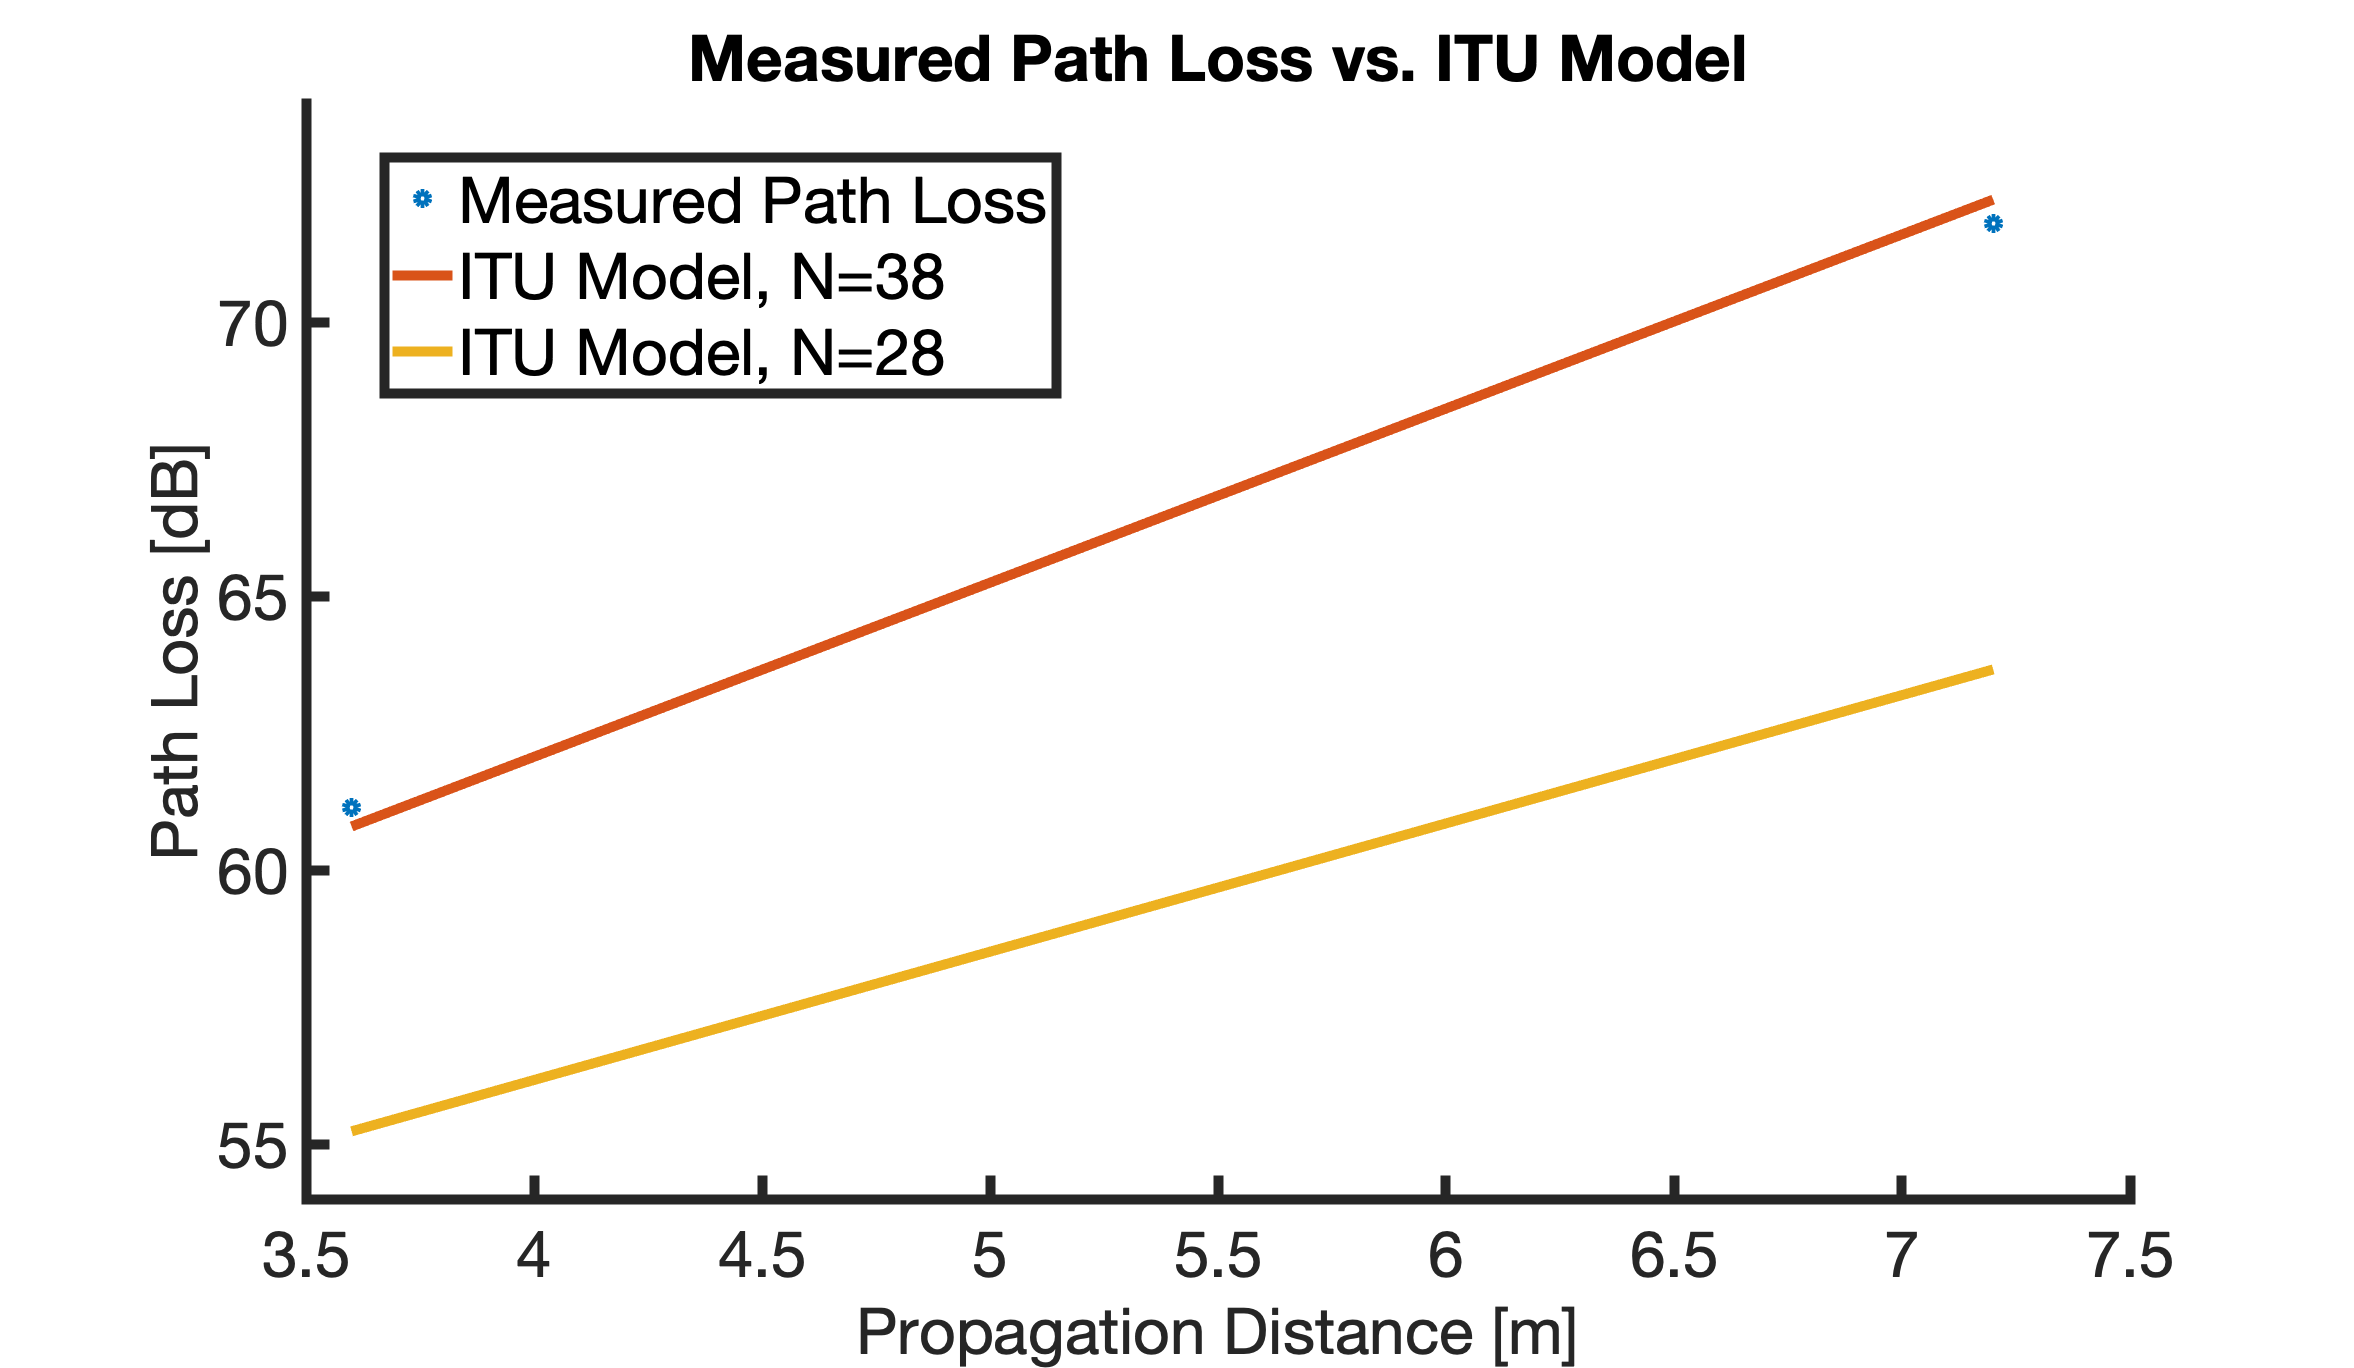
\includegraphics[width=\figW\linewidth]{PathLoss.png}
\caption{Measured path loss vs. estimated path loss from the ITU Indoor Propagations Loss Model, before and after adjusting the power loss coefficient}
\label{fig:path_loss}
\end{center}
\end{figure}


 Other loss factors such as pointing loss and polarisation loss was considered, but measurements showed that the amount of reflections in the room made pointing and polarisation irrelevant to the received power. 
 
The antenna noise density was measured with a spectrum analyser and the estimated value was taken as an average of several single runs. The noise figure of the receiver is included to account for noise added by the radio hardware, with value taken from the data sheet. 

%\subsection{RX Properties}
%\label{sec:rxproperties}
%Some key properties of the received signal is calculated based on the estimated values in the link budget. The BER and $E_b/N_0$ is calculated for the two modulation schemes separately. The bit error rate is calculated for QPSK and QAM-64 by equation \ref{eq:berqpsk} and \ref{eq:berqam} respectively.
%
%\begin{equation}
%\label{eq:berqpsk}
%P_B \approx \frac{1}{2}\erfc\sqrt{\frac{E_b}{N_0}}
%\end{equation}
%
%\begin{equation}
%\label{eq:berqam}
%P_B \approx \frac{2}{\log_2M}\left(1-\frac{1}{M}\right)\erfc\left(\sqrt{\frac{3\log_2M}{2(M-1)}\cdot \frac{E_b}{N_0}}\right)
%\end{equation}





\newpage
% DESIGN DESCRIPTION
% !TEX root = main.tex
\section{Design Description}
\label{sec:design_description}
Figure \ref{fig:block_toplevel} shows how the transmitter and receiver communicates within the system. Block diagrams for the two subsystems are shown in appendix \ref{a:block_diagram}, figure \ref{fig:block_diagram} and \ref{fig:block_diagram_feedback}. The data rate between each block of the data path is indicated with the thin arrows. The behaviour of the system will be explained in this section. 

Because two different modulation schemes are used, the receiver need to know how to decode the incoming data packets. This problem is solved by using two different training sequences in the beginning of each frame. As shown in figure \ref{fig:block_diagram}, after frame sync, the receiver perform a check on the received Barker sequence before de-mapping the symbols. 

In the transmitter, a variable called \textit{Session State} keep the information about what data quality and modulation scheme to use. As figure \ref{fig:block_diagram} indicates, the session state influences several blocks of the TX side of the transmitter. The decision of when to change data quality is left completely to the transmitter. For every received data packet, the receiver computes the number of detected errors and transmit this number back to the transmitter. These BER packets are always transmitted using QPSK-modulation. Based on the received number of detected errors the transmitter decides whether to change session state or not. 

The sound producer and sound consumer contains functionality for handling the sound input and output to the sound card of the computer. They are implemented using the Windows API \cite{WinAPI}. Sound producer reads sound samples from the sound card at full quality (16 bit, 44100 Hz stereo) and writes the samples to a queue accessible for the source encoder. Sound consumer equivalently reads sound samples from a queue controlled by the unpacking block and writes to the computer sound card. 

The source encoder performs lossy compression of the produced sound samples. The bit resolution is reduced to 12 bit per sound sample, and the sampling rate is reduced by a factor 2 or 4 depending on the session state. The source decoder performs the inverse operation, writing 2 or 4 copies of the same sample to the sound consumer.  

In the packing block, sound data is read from the source encoder, a header is added, and the packet is sent to the packet queue. The eight bit packet header consist of a three bit session ID and a five bit packet ID. 

A scrambler is implemented before FEC, which computes a bitwise XOR between a pseudo random bit string and the packet. The bit string used for scrambling is of the same size as the packet itself. The scrambler performs the exact same operation at RX and TX.

The implemented FEC algorithm is Hamming (7,4). The implementation is a fast, pre-written C-code, written by Michael Dipperstein \cite{hamming}. 

The system uses Grey Code for mapping the binary data to a complex vector $z$. The mapping schemes are shown in figure \ref{fig:mapping}.

% !TEX root = main.tex
\begin{figure} 
    \centering
  \subfloat[\label{1a}]{%
  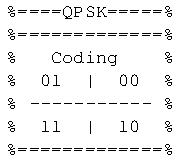
\includegraphics[width=0.3\linewidth]{qpsk_mapping.pdf}
  
}
\\ 
  \subfloat[\label{1b}]{%
    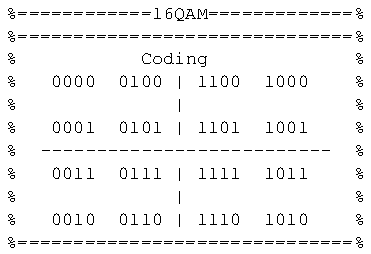
\includegraphics[width=0.6\linewidth]{qam16mapping.pdf}
}

  \caption{Symbol mapping for QPSK (a) and QAM-16 (b) modulated symbols}
  \label{fig:mapping} 
\end{figure}


The training sequence is added to both I and Q symbols in the block \textit{Add Barker}. The training sequence is an appropriate repetition of Barker sequences of length 7 and 13 for QPSK and QAM-16 modulation respectively. The total length of the training sequence is 26 symbols. 

In the last step before transmission, the symbols are upsampled by a factor $\sps$ and filtered with a pulse shaping filter. The filter is Root Raised Cosine with a roll-off factor of 0.3. The same filter is applied as a matched filter in the first step at the receive side before the samples are downsampled again. 

The USRP is configured to transmit continuously with a symbol rate of $\symbolRateQPSK$ symbols per second and transmit arrays of zeros when no data is available. The USRP interface is implemented using the NI-USRP DLL \cite{labviewDLL}.

Symbol synchronisation is done by choosing the sample offset that maximizes the signal energy. 

Frame synchronisation is done by computing the crosscorrelation between the two training sequences and the received symbols. The value of the crosscorrelation is compared to a pre set threshold. The first index that gives a value exceeding this threshold is considered to be the beginning of the frame. After a frame is found, only the frame symbols are passed along to the next block.

\subsection{Frequency and Phase Synchronisation}
The implemented frequency synchronisation algorithm is based on the Mth-power algorithm, which is further improved by using a Kalman filter. Frequency offset is estimated from the training sequence only. The Mth-power algorithm estimates the phase offset of MPSK modulated symbols, by mapping all symbols to the same point in the complex plane. By tracking the angular difference between consecutive symbols, the frequency offset may be estimated. In our case, the QPSK symbols of the training sequence is raised to the 4th power, and the phase is estimated as indicated in figure \ref{fig:mth_pow}.
% !TEX root = main.tex
\begin{figure}[htbp]
\centering
\begin{tikzpicture}
% Grids
\coordinate (origo) at (0,0);
\coordinate (origo_w) at (5.1,0);

\draw[step=0.3cm,gray,very thin] (-1.51,-1.51) grid (1.5,1.5);
\draw[step=0.3cm,gray,very thin] (3.6,-1.51) grid (6.6, 1.5);

% Axis
\draw[thick, ->] (-1.5,0) -- (1.5, 0) node [anchor=north west]{\Re[$z$]};
\draw[thick, ->] (0,-1.5) -- (0,1.5) node [anchor=south west]{\Im[$z$]};
\draw[thick, ->] (3.6,0) -- (6.6, 0) node [anchor=north west]{\Re[$w$]};
\draw[thick, ->] (5.1,-1.5) -- (5.1,1.5) node [anchor=south west]{\Im[$w$]};

\draw[thick] (0.9, 0) ++(0, 2pt) -- ++(0,-4pt) node[font=\scriptsize, yshift=-0.1cm, xshift=-0.1cm]{1};
\draw[thick] (-0.9, 0) ++(0, 2pt) -- ++(0,-4pt) node[font=\scriptsize, yshift=-0.1cm, xshift=-0.1cm]{-1};
\draw[thick] (0, 0.9) ++(2pt, 0) -- ++(-4pt, 0) node[font=\scriptsize, yshift=-0.1cm, xshift=-0.1cm]{1};
\draw[thick] (0, -0.9) ++(2pt, 0) -- ++(-4pt, 0) node[font=\scriptsize, yshift=-0.1cm, xshift=-0.1cm]{-1};

\draw[thick] (6, 0) ++(0, 2pt) -- ++(0,-4pt) node[font=\scriptsize, yshift=-0.1cm, xshift=-0.1cm]{4};
\draw[thick] (4.2, 0) ++(0, 2pt) -- ++(0,-4pt) node[font=\scriptsize, yshift=-0.1cm, xshift=-0.1cm]{-4};
\draw[thick] (5.1, 0.9) ++(2pt, 0) -- ++(-4pt, 0) node[font=\scriptsize, yshift=-0.1cm, xshift=-0.1cm]{4};
\draw[thick] (5.1, -0.9) ++(2pt, 0) -- ++(-4pt, 0) node[font=\scriptsize, yshift=-0.1cm, xshift=-0.1cm]{-4};

% Plot
\draw[blue,fill=blue] (0.9,0.9) circle (2pt) coordinate[](sample);
\draw[blue,fill=blue] (-0.9,0.9) circle (2pt);
\draw[blue,fill=blue] (0.9,-0.9) circle (2pt);
\draw[blue,fill=blue] (-0.9,-0.9) circle (2pt);
\draw[red,fill=red] (0.73,1.043) circle (2pt) coordinate[](sample_err);

\draw[thin, blue] (0,0) -- (sample);
\draw[thin, red] (0,0) -- (sample_err);
\pic [draw, red, ->, angle eccentricity=1.5] {angle = sample--origo--sample_err};
\draw (0.3, 0.3) node[anchor=north west, text=red, yshift=0.2cm]{$\phi$};

\draw[blue,fill=blue] (3.83,0) circle (2pt) coordinate[](sample_w);
\draw[red,fill=red] (4.125,-0.818) circle (2pt) coordinate[](sample_err_w);
\draw[thin, blue] (origo_w) -- (sample_w);
\draw[thin, red] (origo_w) -- (sample_err_w);
\pic [draw, red, ->, angle eccentricity=1.5] {angle = sample_w--origo_w--sample_err_w};
\draw (origo_w) ++(-1.1,-0.35) node[anchor=north west, text=red, yshift=0.2cm]{$4\phi$};

% Other
\draw[thick, ->] (2, 1) .. controls (2.5,1.1) .. (3,1) node[above, anchor=south east, xshift=0.1cm]{$w=z^4$} ;

\end{tikzpicture}
\caption{Illustration the mapping $w=z^4$ which indicates how a phase error in QPSK modulated signal can be observed.}
\label{fig:mth_pow}
\end{figure}

For each received frame, the frequency offset is estimated by the mean of the angular difference between all consecutive symbols of the training sequence. The estimate obtained from a single frame at time $k$  is referred to as $\widetilde{\omega}_k$.  

The accuracy of the estimate is improved by using a Kalman filter. The state of the Kalman filter is the one-dimensional state vector $\omega_k$ which is the true frequency offset between the transmitter and the receiver at time $k$ (i.e. frame $k$). The state is represented by the \textit{a posteriori} state and variance estimate $\widehat{\omega}_{k | k}$ and $\widehat{\sigma}_{k | k}$, where the subscript $n | m$ indicates the estimate of time $n$ given observations up to and including time $m \leq n$. 

The estimate is obtained in two stages, referred to as the \textit{prediction stage} and the \textit{update stage}. In the prediction stage, the \textit{a priori} estimates $\widehat{\omega}_{k | k-1}$ and $\widehat{\sigma}_{k | k-1}$ is obtained by equations \ref{eq:kalman_pred_wk} and \ref{eq:kalman_pred_sigmak}. $\sigma_f$ is the stationary variance of the process noise and must be tuned carefully in order to obtain appropriate convergence speed. In our system $\sigma_f$ was set to $0.8\cdot 10^{-6}$.  

\begin{gather}
\widehat{\omega}_{k | k-1} = \widehat{\omega}_{k-1 | k-1}  \label{eq:kalman_pred_wk} \\
\widehat{\sigma}_{k | k-1} = \widehat{\sigma}_{k-1 | k-1} + \sigma_f \label{eq:kalman_pred_sigmak} 
\end{gather} 

In the update stage, the \textit{a posteriori} estimates $\widehat{\omega}_{k | k}$ and $\widehat{\sigma}_{k | k}$ is obtained by equations \ref{eq:kalman_up_wk} and \ref{eq:kalman_up_sigmak}. $\widetilde{\omega}_k$ and $\widetilde{\sigma}_{k}$ is the observed frequency offset and estimated observation noise at time $k$ respectively.

\begin{gather}
\widehat{\omega}_{k | k} = \widehat{\omega}_{k | k-1} + \frac{\widehat{\sigma}_{k | k-1}}{\widehat{\sigma}_{k | k-1} + \widetilde{\sigma}_{k}} ( \widetilde{\omega}_{k} - \widehat{\omega}_{k | k-1} )  \label{eq:kalman_up_wk} \\
\widehat{\sigma}_{k | k} = \widehat{\sigma}_{k | k-1} \frac{\widetilde{\sigma}_{k}}{\widetilde{\sigma}_{k} + \widehat{\sigma}_{k | k-1}  } \label{eq:kalman_up_sigmak} 
\end{gather} 

After the estimates $\widehat{\omega}_{k | k}$ and $\widehat{\sigma}_{k | k}$ is obtained, $\widehat{\omega}_{k | k}$ is applied to each symbol in frame $k$. The phase offset is then estimated as the mean of the angular deviation between the training sequence of the received symbols, and the ideal Barker sequence.




% DESIGN MOTIVATION
\section{Design Motivation}
\label{sec:design_motivation}

As stated in section \ref{sec:introduction}, the purpose of the proposed system is to demonstrate a radio system with adaptable data rate and this is the background for all design choices that is made. 

% VERIFICATION
% !TEX root = main.tex
\section{Measurements and Verification}
\label{sec:verification}



% CONCLUSION
% !TEX root = main.tex
\section{Conclusion}
\label{sec:conclusion}
The design and implementation of a radio communication system for broadcasting of speech with adaptable data rate is presented. The system adapts the transmitted data rate to the state of the radio channel by evaluating detected bit error at the receiver. The transmitted data rate is varied by a factor 2 by switching modulation format between QPSK and QAM-16. 

The system was verified in an indoor environment with a transmission distance of 1 meter and variations in the radio channel is simulated by adjusting the transmit power. The system transmit at high data rate ($520,8$ kb/s) when using QAM-16 modulated symbols at $\measPWR$ dBm and low data rate ($249$ kb/s) for QPSK at $\measPWRbad$ dBm. Bit error rates of \measBERQAMGood and \measBERQPSKBad was measured at high and low data rate respectively.

The high BER for QAM-16 modulation makes the effect of adaptable quality hardly audible, because of the high noise level when transmitting at high data rate. The adaptable quality feature is however interesting in itself and this demonstration shows a working ``proof of concept''. By adapting the transmitted data rate to the state of the radio channel, the system yields a better utilization of available resources. This two-level adaption could be extended to several levels for higher performance in future improvements.

% BIBLIOGRAPHY
\bibliographystyle{IEEEtran}
\bibliography{references}

% APPENDICES
\appendices

\section{Block Diagram}
\label{a:block_diagram}
% !TEX root = main.tex
\begin{figure*}[htbp]
\centering
\begin{tikzpicture}[                
                    box/.style={
            		draw,
			thick,
            		text centered,
            		minimum width=1cm,
            		minimum height=1cm,
			font=\scriptsize,
			align=center,
			anchor=center,
            	}, decision/.style={
			draw,
			diamond,
			thick,
			align=center,
            		minimum width=1cm,
            		minimum height=1cm,
			font=\scriptsize,
			anchor=center,	
		}, ]
	
% ------ USRP ------- %
\filldraw[fill=black!20!white, draw=black!20!white, opacity=0.5] (13, 2.5) rectangle (15,-6.5);
\draw (14, 2.5) node[anchor=north, align=center]{RF \\ Hardware};

% -------- TX --------- %
\filldraw[fill=black!10!white, draw=black!10!white, opacity=0.5] (-2.5,2.5) rectangle (13,-6.5);

\draw (-2.5,2.5) node[anchor=north west]{TX - Software};
% Draw boxes
\draw 
(1.25, 1.5) node[box, anchor=west, minimum width=9.75cm, font=\footnotesize](state){Session State}

(0,0) node[box](sound_prod){Sound \\ producer} 
(1.75,0) node[box](source_enc){Source \\ encoder} 
(3.5,0) node[box](packing_tx){Packing} 
(5.25,0) node[box](scramble_tx){Scrambler} 
(7,0) node[box](fec_tx){FEC} 
(8.75,0) node[box](symbol_mapping_tx){Symbol \\ mapping} 
(10.5,0) node[box](barker_tx){Add \\ Barker} 
(12.25,0) node[box](pulse_shape_tx){Pulse \\ shaping} 
(14,0) node[box](usrp_tx){USRP \\ TX} 
;


\draw [->, thick] (sound_prod.east) -- node[below, yshift=-1.6cm](r0){} node[](r00t){} (source_enc.west);
\draw [->, thick] (source_enc.east) -- node[](r01t){} (packing_tx.west);
\draw [->, thick] (packing_tx.east) --  node[](r02t){}(scramble_tx.west);
\draw [->, thick] (scramble_tx.east) -- node[](r03t){} (fec_tx.west);
\draw [->, thick] (fec_tx.east) --  node[](r04t){}(symbol_mapping_tx.west);
\draw [->, thick] (symbol_mapping_tx.east) -- node[](r05t){} (barker_tx.west);
\draw [->, thick] (barker_tx.east) -- node[](r06t){} (pulse_shape_tx.west);
\draw [->, thick] (pulse_shape_tx.east) -- node[](r07t){} (usrp_tx.west);

% State lines
\draw [<-, thick] (source_enc.north) -- ++(0, 0.5);
\draw [<-, thick] (packing_tx.north) -- ++(0, 0.5); 
\draw [<-, thick] (symbol_mapping_tx.north) -- ++(0, 0.5); 
\draw [<-, thick] (barker_tx.north) -- ++(0, 0.5);

% DATA RATES
\draw
(r0) node[above, font=\tiny, align=center](r1){$\rawDataRate$ \\ Mb/s}
++(1.75, 0) node[above, font=\tiny, align=center](r2){$\sourceDataRateQPSK  /  \sourceDataRateQAM$\\ kb/s}
++(1.75, 0) node[above, font=\tiny, align=center](r3){$\packetDataRateQPSK  /  \packetDataRateQAM$\\ kb/s}
++(1.75, 0) node[above, font=\tiny, align=center](r4){$\fecDataRateQPSK  /  \fecDataRateQAM$\\ kb/s}
++(1.7, 0) node[above, font=\tiny, align=center](r5){$\symbolMapRateQPSK  /  \symbolMapRateQAM$\\ ksymb/s}
++(1.5, 0) node[above, font=\tiny, align=center](r6){$\barkerRateQPSK  /  \barkerRateQAM$\\ ksymb/s}
++(1.3, 0) node[above, font=\tiny, align=center](r7b){$\symbolRateQPSK$\\ ksymb/s}
++(1.3, 0) node[above, font=\tiny, align=center](r7){$\sampleRateQPSK / \sampleRateQAM$\\ Msamp/s}
++(1.1, 0) node[above, font=\tiny, align=center](r8){$\USRPSampleRate$\\ Msamp/s}
;


% -------- RX --------- %
\draw (-2.5,-1.5) node[anchor=north west]{RX - Software};
% Draw boxes
\draw 
(-1.5,-3) node[box](sound_cons){Sound \\ consumer} 
(0,-3) node[box](source_decode){Source \\ decoder} 
(1.5,-3) node[box](unpack_rx){Unpacking} 
(3,-3) node[box](scramble_rx){Scrambler} 
(4.5,-3) node[box](fec_rx){FEC \\ decoding} 
(6,-3) node[box](demap_rx){De- \\ mapping} 
(7.5,-3) node[box](freq_sync_rx){Frequency \\ and \\ phase \\ sync} 
(9,-3) node[box](frame_sync_rx){Frame \\ sync} 
(10.5,-3) node[box](symb_sync_rx){Symbol \\ sync} 
(12,-3) node[box](filter_rx){Matched \\ filter} 
(14,-3) node[box](usrp_rx){USRP \\ RX} 
;

\node [decision, below of=frame_sync_rx, yshift=-1cm] (barker_length_dec) {Barker \\ length?};
\node [box, minimum height=0cm, left of=barker_length_dec, yshift=0.5cm, xshift=-0.5cm](qpsk_out){Modulation \\ QPSK};
\node [box, minimum height=0cm, left of=barker_length_dec, yshift=-0.5cm, xshift=-0.5cm](qam_out){Modulation \\ QAM-64};
\node [box, below of=fec_rx, yshift=-1cm,](send_error){Send BER \\ to \\ transmitter};

\draw [->, thick] (usrp_tx.south) -- ++ (-0.1, -1) -- ++(0.2, 0.2) node[right, align=center, font=\scriptsize, anchor=west, xshift=-0.1cm]{Speech \\ data} -- (usrp_rx.north);

\draw [->, thick] (usrp_rx.west) -- node[](r09r){} (filter_rx.east);
\draw [->, thick] (filter_rx.west) -- node[](r08r){} (symb_sync_rx.east);
\draw [->, thick] (symb_sync_rx.west) -- node[](r07r){} (frame_sync_rx.east);
\draw [->, thick] (frame_sync_rx.west) -- node[](r06r){} (freq_sync_rx.east);
\draw [->, thick] (freq_sync_rx.west) -- node[](r05r){} (demap_rx.east);
\draw [->, thick] (demap_rx.west) -- node[](r04r){} (fec_rx.east);
\draw [->, thick] (fec_rx.west) -- node[](r03r){} (scramble_rx.east);
\draw [->, thick] (scramble_rx.west) -- node[](r02r){} (unpack_rx.east);
\draw [->, thick] (unpack_rx.west) -- node[](r01r){} (source_decode.east);
\draw [->, thick] (source_decode.west) -- node[](r00r){} (sound_cons.east);

\coordinate [below of=demap_rx, xshift=0.2cm, yshift=0.5cm](qpsk_in) {};
\coordinate [below of=demap_rx, xshift=-0.2cm, yshift=0.5cm](qam_in) {};

\draw [->, thick] (frame_sync_rx.south) -- node[right, font=\scriptsize, align=center] {Detected \\ Barker} (barker_length_dec.north);
\draw [->, thick] (barker_length_dec.west) ++(0.5,0.5) -- node[above, font=\scriptsize]{7} (qpsk_out.east);
\draw [->, thick] (barker_length_dec.west) ++(0.5,-0.5) -- node[below, font=\scriptsize]{13} (qam_out.east);
\draw [->, thick] (qpsk_out.west) -| (qpsk_in);
\draw [->, thick] (qam_out.west)  -| (qam_in);
\draw [->, thick] (fec_rx.south)  -- node[left, font=\scriptsize, align=center]{Number of \\ detected \\ errors} (send_error.north);

% Data rate arrows
\draw[->, thin] (r1.north) to[out=90,in=270] (r00t);
\draw[->, thin] (r2.north) to[out=90,in=270] (r01t);
\draw[->, thin] (r3.north) to[out=90,in=270] (r02t);
\draw[->, thin] (r3.north)++(0.3, 0) to[out=45,in=270] (r03t);
\draw[->, thin] (r4.north)++(0.3, 0) to[out=45,in=270] (r04t);
\draw[->, thin] (r5.north)++(0.3, 0) to[out=45,in=270] (r05t);
\draw[->, thin] (r6.north)++(0.3, 0) to[out=45,in=270] (r06t);
\draw[->, thin] (r7.north)++(0.5, 0) to[out=35,in=270] (r07t);
\draw[->, thin] (r8.east) -- ++(0.3, 0);

\draw[->, thin] (r8.south)++(0.1,0) to[out=-70,in=90] (r09r);
\draw[->, thin] (r8.south)++(-0.3,0) to[out=210,in=90] (r08r);
\draw[->, thin] (r7b.south)++(-0.2,0.05) to[out=250,in=90] (r07r);
\draw[->, thin] (r6.south)++(-0.4, 0.2) to[out=210,in=90] (r06r);
\draw[->, thin] (r5.west)++(0.2, -0.1) to[bend right] (r05r);
\draw[->, thin] (r4.west)++(0.4, -0.1) to[bend right] (r04r);
\draw[->, thin] (r3.south)++(-0.2, 0) to[out=230,in=90] (r03r);
\draw[->, thin] (r3.west)++(0.2, -0.1) to[out=200,in=90] (r02r);
\draw[->, thin] (r2.west)++(0.2, -0.1) to[out=200,in=90] (r01r);
\draw[->, thin] (r1.south)++(-0.2,0) to[out=210,in=90] (r00r);


\end{tikzpicture}

\caption{Block diagram of data packet system. This block diagram shows the forward path of the system, where speech data is being transmitted. Data rates for Low/High data quality is indicated on each arrow.}
\label{fig:block_diagram}
\end{figure*}
% !TEX root = main.tex
\begin{figure*}[htbp]
\centering
\begin{tikzpicture}[                
                    box/.style={
            		draw,
			thick,
            		text centered,
            		minimum width=0.8cm,
            		minimum height=0.8cm,
			font=\scriptsize,
			align=center,
			anchor=center,
            	}, decision/.style={
			draw,
			diamond,
			thick,
			align=center,
            		minimum width=0.8cm,
            		minimum height=0.8cm,
			font=\tiny,
			anchor=center,	
		}, ]
	
% ------ USRP ------- %
\filldraw[fill=black!20!white, draw=black!20!white, opacity=0.5] (13, 1.5) rectangle (15,-6.5);
\draw (14, 1.5) node[anchor=north, align=center]{RF \\ Hardware};

% -------- TX --------- %
\filldraw[fill=black!10!white, draw=black!10!white, opacity=0.5] (-1.5,1.5) rectangle (13,-6.5);
\draw (-1.5,1.5) node[anchor=north west]{TX - Software};
% Draw boxes
\draw 
(0,0) node[](detected_errors){} 
(2,0) node[box](packing_tx){Packing} 
(4,0) node[box](scramble_tx){Scrambler} 
(6,0) node[box](fec_tx){FEC} 
(8,0) node[box](symbol_mapping_tx){Symbol \\ mapping} 
(10,0) node[box](barker_tx){Add \\ Barker} 
(12,0) node[box](pulse_shape_tx){Pulse \\ shaping} 
(14,0) node[box](usrp_tx){USRP \\ TX} 
;

\draw [->, thick] (detected_errors.east) -- node[above, font=\footnotesize, align=center]{Detected \\ Errors} (packing_tx.west);
\draw [->, thick] (packing_tx.east) -- (scramble_tx.west);
\draw [->, thick] (scramble_tx.east) -- (fec_tx.west);
\draw [->, thick] (fec_tx.east) -- (symbol_mapping_tx.west);
\draw [->, thick] (symbol_mapping_tx.east) --  (barker_tx.west);
\draw [->, thick] (barker_tx.east) -- (pulse_shape_tx.west);
\draw [->, thick] (pulse_shape_tx.east) -- (usrp_tx.west);


% -------- RX --------- %
\draw (-1.5,-1.5) node[anchor=north west]{RX - Software};
% Draw boxes
\draw
(1.5,-3) node[box](unpack_rx){Unpacking} 
(3,-3) node[box](scramble_rx){Scrambler} 
(4.5,-3) node[box](fec_rx){FEC \\ decoding} 
(6,-3) node[box](demap_rx){De- \\ mapping} 
(7.5,-3) node[box](freq_sync_rx){Frequency \\ and \\ phase \\ sync} 
(9,-3) node[box](frame_sync_rx){Frame \\ sync} 
(10.5,-3) node[box](symb_sync_rx){Symbol \\ sync} 
(12,-3) node[box](filter_rx){Matched \\ filter} 
(14,-3) node[box](usrp_rx){USRP \\ RX} 
;

\draw [->, thick] (usrp_tx.south) -- ++ (-0.1, -1) -- ++(0.2, 0.2) node[right, align=center, font=\scriptsize, anchor=west, xshift=-0.2cm, yshift=0.1cm]{Detected \\ errors} -- (usrp_rx.north);\draw [->, thick] (usrp_rx.west) -- (filter_rx.east);
\draw [->, thick] (filter_rx.west) -- (symb_sync_rx.east);
\draw [->, thick] (symb_sync_rx.west) -- (frame_sync_rx.east);
\draw [->, thick] (frame_sync_rx.west) -- (freq_sync_rx.east);
\draw [->, thick] (freq_sync_rx.west) -- (demap_rx.east);
\draw [->, thick] (demap_rx.west) -- (fec_rx.east);
\draw [->, thick] (fec_rx.west) -- (scramble_rx.east);
\draw [->, thick] (scramble_rx.west) -- (unpack_rx.east);
\draw[->, thick] (demap_rx.south) ++(1, -0.7) -- node[above, font=\scriptsize]{QPSK} ++(-1, 0) -- (demap_rx.south);


\node [decision, below of=unpack_rx, yshift=-0.5cm, font=\scriptsize] (change_state) {Change \\ state?};
\node [box, below of=change_state, yshift=-0.5cm, minimum height=0] (do_nothing) {Do nothing};
\node [box, left of=change_state, xshift=-0.8cm, minimum height=0] (do_change) {Change \\ state};

\draw [->, thick] (unpack_rx.south) -- (change_state.north);
\draw [->, thick] (change_state.south) -- node[right, font=\scriptsize, yshift=3]{No} (do_nothing.north);
\draw [->, thick] (change_state.west) -- node[above, font=\scriptsize]{Yes} (do_change.east);


\end{tikzpicture}

\caption{Block diagram of BER packet system. This sub-system constitutes the feedback path where the receiver transmit information about detected error rate back to the transmitter.}
\label{fig:block_diagram_feedback}
\end{figure*}

\end{document}